%Punchline!

%make plot of delta [C/N] versus R0(1D), color code observed binned points by mass of the star

Given the measured amounts of mixing described in Section \ref{sec:obs} and the reduced density ratios $r$ computed for stars of various masses and metallicities described in Section \ref{sec:mesa_results}, it is now possible to compare the observations to the predictions of various thermohaline models from Section \ref{sec:formalism} and to assess whether the observed mixing is qualitatively consistent with any such theoretical prescription.
%that which would be driven by the thermohaline instability.
%
We show in Figure \ref{Fig:punchline} the corrected changes in [C/N] compared to the inferred reduced density ratios on axes analogous to those of Figure \ref{fig:parameterization_compare}, where the y axis represented the rate of mixing. % theoretical predictions were first introduced}. \textbf{
The four panels correspond to the four modeling configurations described in Section \ref{sec:mesa_experiment}. %\textcolor{red}{[Feel free to drop this, but: is there an easy way to remind the reader why the y axis on this figure is analogous to the y axis on figure 1? -AF]}

We first note that the observed trends are not strongly sensitive to the assumed 1D mixing model: mixing decreases with increasing reduced density ratio regardless of parameterization.
%
Besides this, the data show both similarities and differences compared to the theoretical predictions, reproduced in Figure \ref{Fig:compare} for comparison. A key finding is that the observed mixing is strongly correlated with the fluid parameters as predicted; this is true for stars with different masses and metallicities but similar reduced density ratios. %\textbf{This is} consistent with theoretical predictions under the simplifying assumption that the mixing efficiency and magnetic field are not varying strongly with mass or metallicity. 
We observe a decrease in the amount of mixing as the density ratio increases, which is consistent with standard 1D prescriptions of thermohaline mixing but inconsistent with the prescription from Harrington \& Garaud 2019, which was informed by magnetohydrodynamic simulations. %the prescription informed by 3D magnetohydrodynamic
%simulations that include strong magnetic fields \textcolor{red}{[I prefer ``" because we don't want to say ``it's not magnets", we just want to say ``it's not the trend HG19 said magnets produce" and I think that's an important distinction. If this change is accepted, I think the part between ``consistent with" and ``but inconsistent with" also needs some slight tweaking. -AF]}.
We also find that the range of average reduced density ratios probed by the observational data we have available here is much smaller than the range of density ratios simulated by and studied within the theoretical 3D fluid dynamics community \citep[e.g.][]{brown_etal_2013}, although we note that the full range of ratios do appear in each individual simulation (See Appendix \ref{app:movie}).% \textcolor{red}{[we should point out that: it's not that larger r's don't ever appear in our MESA models, since they do (see appendix C), it's just that the metric we're focusing on here appears to be probing (or something) these smaller r's. -AF]}. 
 %As such, we must be cognizant of the limitations of our analysis; for instance, the observations do not probe the high-$r$ regimes \sout{where magnetic fields are most important} \textbf{which are presumably important for determining how the thermohaline-unstable region propagates until it reaches the convective envelope [-AF]}. 


%note that the scatter is also important here- if the mixing actually depends on B field, and that depends randomly on the star (or on the stellar M/Z combo on average), then stars of the same R0 should have a range of mixi-ness. If R0 is the only parameter that matters, then mixing should strongly correlate with R0 with only minimal/ observational measurement scatter. 

%FIGURE solar---------------------------------------------------
\begin{figure*}[!tb]
\begin{center}
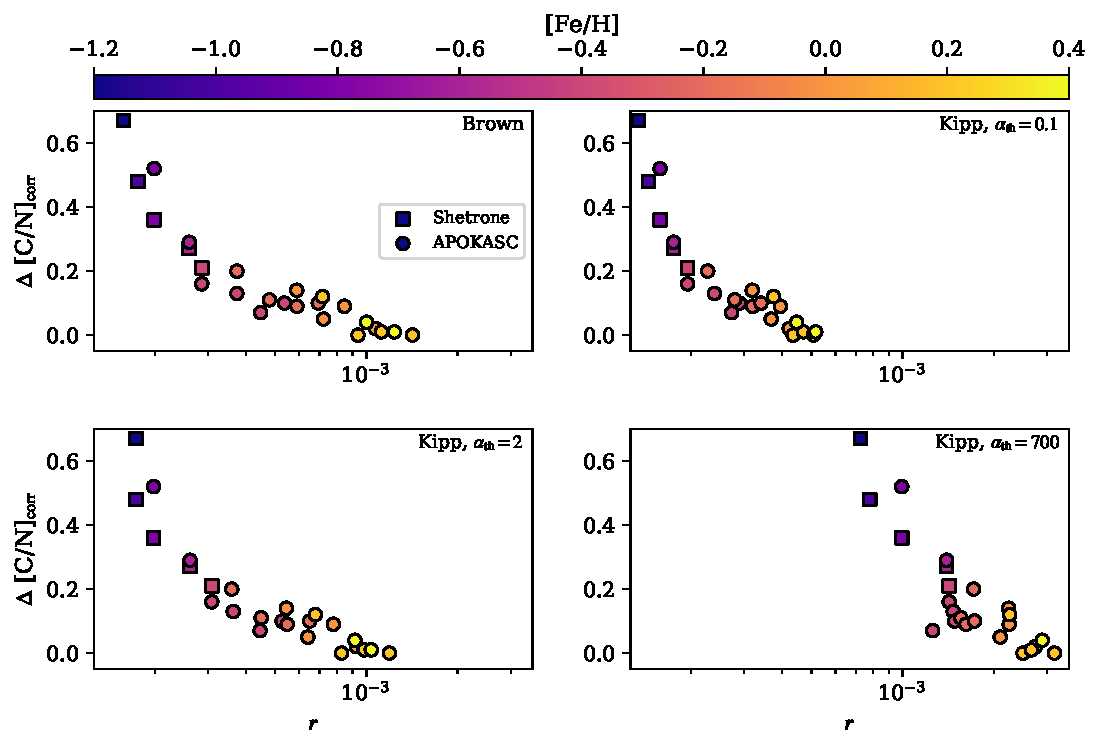
\includegraphics[width=\textwidth]{mixing_vs_r.pdf}%[width=9cm, clip=true, trim=1in 1in 1in 1in]{./Figs/omgcomp.eps}
\caption{Corrected measurements of the change in [C/N] near the red giant branch bump are compared to the reduced density ratio inferred from one-dimensional models using various thermohaline mixing prescriptions (Brown, Kippenhahn $\alpha_{\rm th}=0.1$, Kippenhahn $\alpha_{\rm th}=0.2$,Kippenhahn $\alpha_{\rm th}=0.700$). Observations are color coded by the metallicity bin of each data point. In general, there is a clear correlation between these parameters, suggesting that the observed mixing may indeed be related to %\textcolor{red}{[``related to" feels weak given how awesome of a result this is, is there a fair way to strengthen it a little? -AF]} 
the unstable mean molecular weight gradient. Mixing and the reduced density ratio $r$ are inversely correlated, which is consistent with hydrodynamic thermohaline prescriptions. %\sout{More mixing is observed when the fluid is more \textbf{unstable to the thermohaline instability [can this be said a different way?]}; this is consistent with standard theories of thermohaline mixing.} 
%We note that the observations do not probe high values of the reduced density ratios, which is where magnetic fields are most important. \textcolor{red}{[I am in favor of striking out this last sentence because the reader could take from this that we claim magnetic fields do not matter, when in fact this range of r values is still in the regime where HG19 says magnetic fields do matter -AF]}
\label{Fig:punchline}
}
\end{center}
\end{figure*}

\begin{figure*}[!tb]
\begin{center}
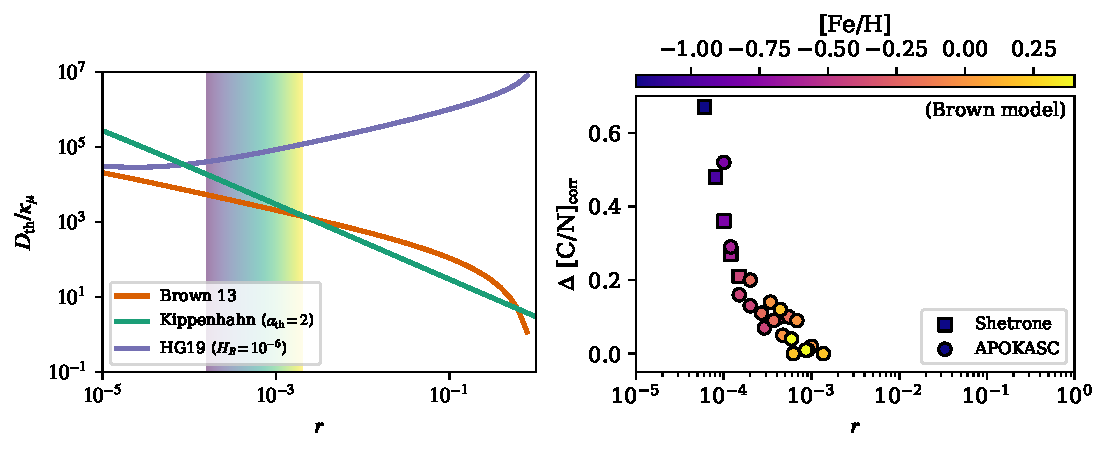
\includegraphics[width=\textwidth]{punchline.pdf}
\caption{\textbf{Left:} A reproduction of Figure \ref{fig:parameterization_compare} showing the predicted rate of mixing versus the reduced density ratio in various prescriptions of thermohaline mixing, including hydrodynamic (orange, green) and magnetohydrodynamic (purple) models. \textbf{Right:} The observed extra mixing near the red giant branch bump as a function of the reduced density ratio inferred from one dimensional stellar evolution models. While the conversion from the change in a mixing diagnostic to the fluid mixing rate is not trivial, and therefore we do not attempt it here, we note that the observed mixing amounts are strongly negatively correlated with $r$, with stars probing on average a relatively narrow range of the regime formally unstable to thermohaline mixing. }
\label{Fig:compare}
\end{center}
\end{figure*}


